\documentclass[../main.tex]{subfiles}

\graphicspath{{../images/}}

\begin{document}
\pagestyle{fancy}
\lhead{Lecture 19: 11/5/24}
\chead{Chapter 6}
\rhead{PHYS 421}

\section{Magnetic Fields in Matter}
\barh \vspace{1em}

\subsection{Magnetization}

\subsubsection{Paramagnets, Diamagnet, Ferromagnets}

\subsubsection{Forces and Torques on Magnetic Dipoles}
Using $\vb F = I \int \dd{\vb l} \times \vb B$ we can find the directions of the forces on each section
of the current loop

\begin{figure}[ht]
    \centering
    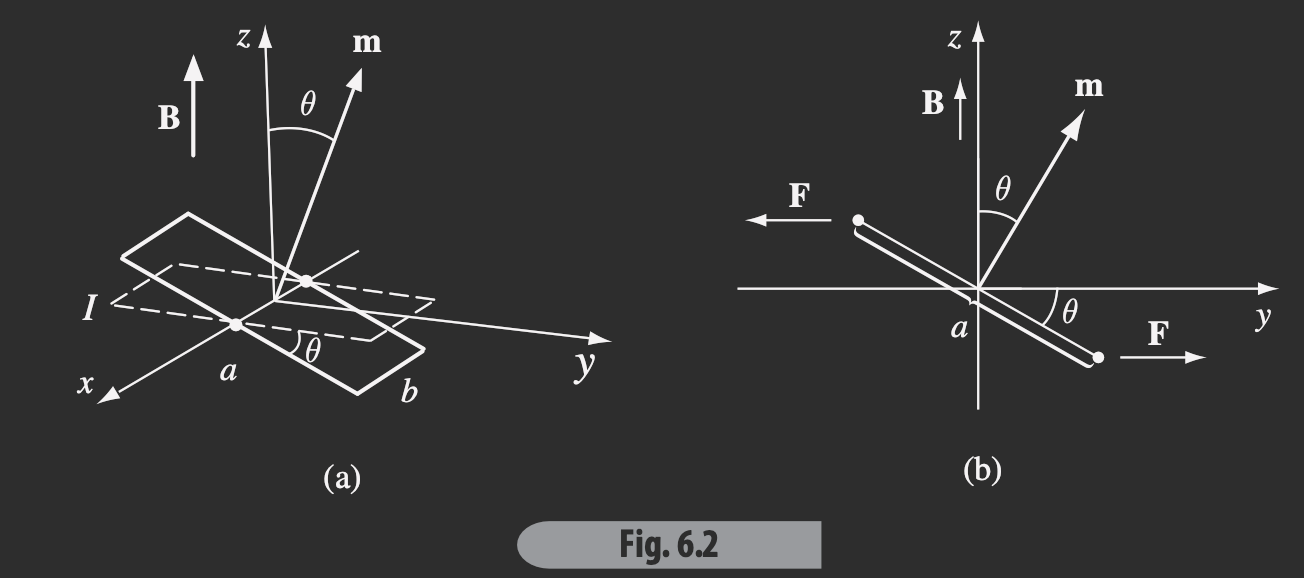
\includegraphics[width=0.8\textwidth]{fig6_2.png}
    \caption{Magnetic field due to a current loop}
    \label{fig:gr6_2}
\end{figure}

Since the sum of the forces $\sum \vb F = 0$ so the magnitude of force on each segment is
\begin{align*}
    F = I b B
\end{align*}
and the torque on the loop is
\begin{align*}
    \vb N = a F \sin\theta \vu{x}
\end{align*}
Or
\begin{align*}
    \vb N &= I a b B \sin\theta \vu{x} \qusing m = I a b \\
    \vb N &= \vb m \cross \vb B
\end{align*}
which encapsulates the defintion of ``paramagnetism'' i.e. the magnetic moments align with the magnetic field.
This is similar to the electric form
\begin{align*}
    \vb N_E = \vb p \cross \vb E
\end{align*}

\paragraph{\dots in a uniform field} The net force $\to$ 0
\begin{align*}
    \vb F = I \oint \dd{\vb l} \cross \vb B = 0
\end{align*}

\newpage
\paragraph{non-uniform field}
\begin{figure*}[ht]
    \centering
    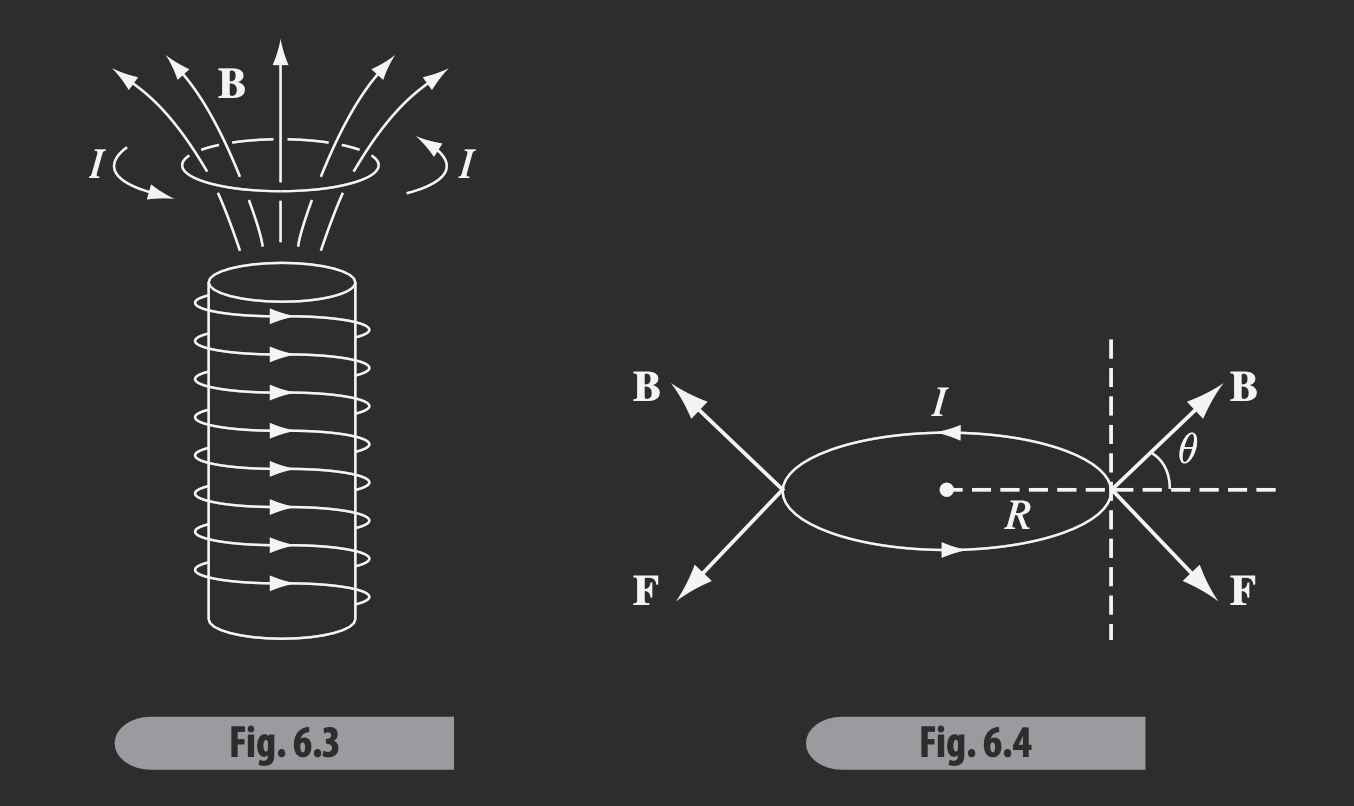
\includegraphics[width=0.8\textwidth]{fig6_3_4.png}
    \caption{Solenoid}
    \label{fig:gr6_3}
\end{figure*}

Using RHR we can see that the horizontal components cancel out from symmetry and we are left with a
downward force on the dipole with magnitude
\begin{align*}
    \abs{\vb F} = 2\pi R I B \sin\theta
\end{align*} At the other end of the dipole, the force will be upwards;
so for the pure dipole
\begin{align*}
    \vb F_B = \grad (\vb m \cdot \vb B) \\
    \vb F_E = \grad (\vb p \cdot \vb E)
\end{align*}

\begin{figure*}[ht]
    \centering
    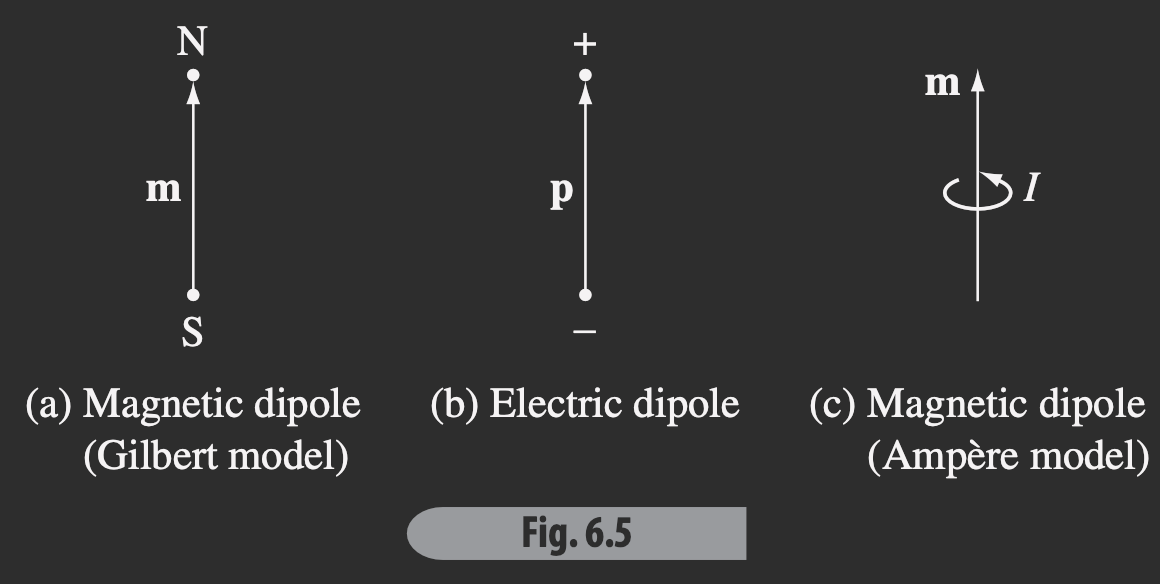
\includegraphics[width=0.8\textwidth]{fig6_5.png}
    \caption{Early models of magnetism}
    \label{fig:gr6_5}
\end{figure*}
From the electric dipole, we could easiliy infer a magnetic dipole or ``Gilbert'' model.

\newpage
\subsubsection{Effect of B on atomic orbitals}

For an electron circulating a nucleus,
\begin{itemize}
    \item Period $T = 2\pi R /v$
    \item $\sim$ stead current $I = -e/T = -e v / (2\pi R)$
    \item Thus a magnetic moment $\vb m = I \vb a = I \pi R^2 (-\vu z) = -\frac{1}{2} ev R\vu z$
\end{itemize}
The centripetal orbital force keeping the electron in orbit is entirely due to the coulomb force
\begin{align*}
    \vb F_\text{orb} &= \vb F_\text{coul} \\
    m_e \frac{v^2}{R} = \ke \frac{e^2}{R^2}
\end{align*}

\begin{figure*}[ht]
    \centering
    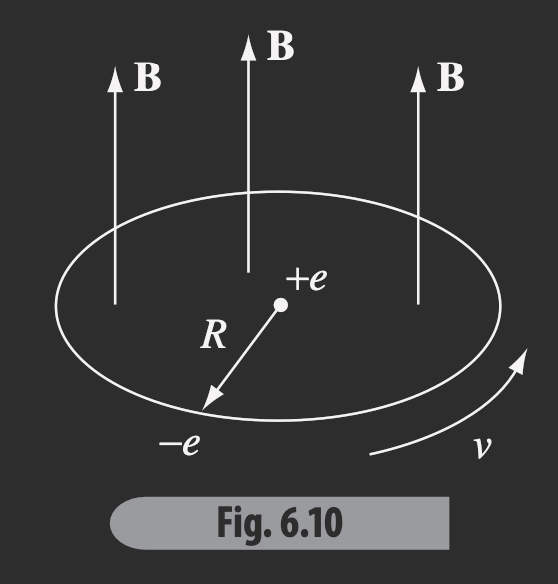
\includegraphics[width=0.4\textwidth]{fig6_10.png}
    \caption{Magnetic field due to an electron}
    \label{fig:gr6_10}
\end{figure*}
From the LHR (for electron) the force points inwards, so
\begin{align*}
    \ke \frac{e^2}{R^2} + ev' B &= m_e \frac{v^2}{R} \\
    \implies ev'B = \frac{mv'^2}{R} - \frac{mv^2}{R} &= \frac{m}{R} (v'^2 - v^2) \\
    &= \frac{m}{R} (v + v')(v' - v) \qusing v' - v = \delta v
\end{align*}
where
\begin{align*}
    \delta v = \frac{ev'B}{m/R} \frac{1}{v' + v} \approx \frac{eRB}{2} \quad v' \approx v
\end{align*}
Using
\begin{align*}
    \vb m = -\frac{1}{2} e v R \vu z \implies \delta m = -\frac{e}{2} R \delta v \vu z = -\frac{e^2 R^2}{4m_e} \vb B 
\end{align*}
This opposite alignment of the magnetic moment is called ``diamagnetism''. Andre Geim shared the Ig Nobel prize for levitating a frog in a magnetic field \href{https://en.wikipedia.org/wiki/Ig_Nobel_Prize#:~:text=The%202000%20Ig%20Nobel%20Prize,Prize%20in%20Physics%20in%202010.}{Wiki}.

\lhead{Lecture 20: 11/7/24}
\subsubsection{Magnetization}
The magnetization is defined by the vector quantity
\begin{align*}
    \vb M = \textrm{magnetic dipole moment/unit volume}
\end{align*}
which is analagous to the electric polarization $\vb P$: 
\subsection{The field of a magnetized object}
\subsubsection{Bound Currents}
The field produced by $\vb M$? For each tiny dipole moment
\begin{align*}
    \vb m = \vb M \dd{\tau} 
\end{align*}
we can use a vector potential
\begin{align*}
    \vb A_m (\vb r) = \frac{\mu_0}{4\pi} \frac{\vb m \cross \vu*\scriptr}{\scriptr^2}
\end{align*}
So the total vector potential (using product rule 7 [insert ref]) and $\grad'{\frac{1}{\scriptr}} = -\frac{\vu*\scriptr}{\scriptr^2}$
\begin{align*}
    \vb A_\text{tot} (\vb r) &= \frac{\mu_0}{4\pi} \int \frac{\vb M(\vb r') \cross \vu*\scriptr}{\scriptr^2} \dd{\tau'} \\
    &= \frac{\mu_0}{4\pi} \int \vb M(\vb r') \cross \grad'{\frac{1}{\scriptr}} \dd{\tau'} \\
    &= \frac{\mu_0}{4\pi} \qt(
        \int \frac{1}{\scriptr} \qt[
            \grad' \cross \vb M(\vb r') 
        ] \dd{\tau'} - \int \grad' \cross \qt[
            \frac{\vb M(\vb r')}{\scriptr}
        ] \dd{\tau'}
    )
\end{align*}
where the second term is
\begin{align*}
    - \int \grad' \cross \qt[
        \frac{\vb M(\vb r')}{\scriptr}
    ] \dd{\tau'} &= \oint \frac{1}{\scriptr} \qt[
        \vb M(\vb r') \cross \dd{\vb a'}
    ] 
\end{align*}
from Stokes' theorem of sorts. The two integrals represent the volume and surface current
\begin{align*}
    \vb J_b &\equiv \grad \cross \vb M \qquad \vb A \sim \int \frac{\vb J_b}{\scriptr} \dd{\tau} \\
    \vb K_b &\equiv \vb M \cross \vu n \qquad \vb A \sim \oint \frac{\vb K_b}{\scriptr} \dd{a}
\end{align*}
so
\begin{align*}
    \vb A(\vb r) = \frac{\mu_0}{4\pi} \int \frac{\vb J_b}{\scriptr} \dd{\tau'} + \frac{\mu_0}{4\pi} \oint \frac{\vb K_b}{\scriptr} \dd{a'}
\end{align*}

\paragraph{Example} Find $\vb B$ of a uniformly magnetized sphere 
\begin{figure*}[ht]
    \centering
    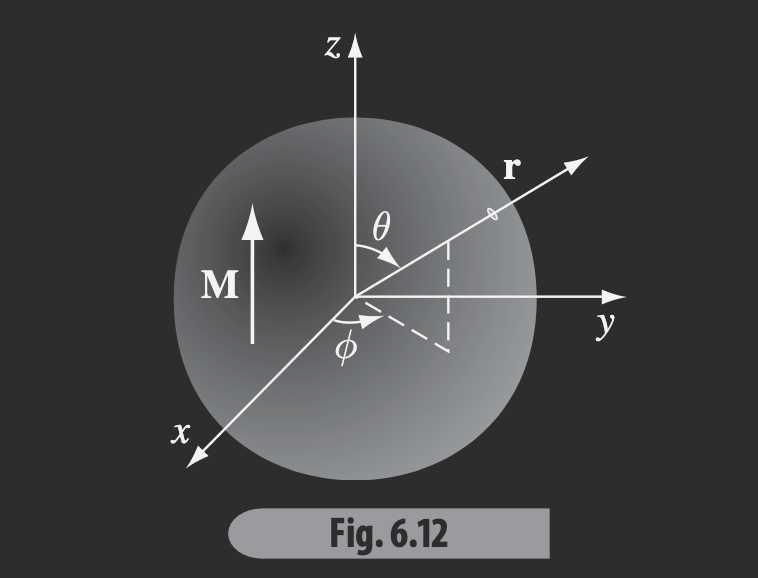
\includegraphics[width=0.4\textwidth]{fig6_12.png}
    \caption{Magnetized sphere}
    \label{fig:gr6_6}
\end{figure*}

Thre curl of a constant vector is zero so
\begin{align*}
    \vb J_b = \grad \cross \vb M = 0
\end{align*}
and for the surface current, we can see that the cross product is always in the azimuthal direction:
\begin{align*}
    \vb K_b = \vb M \cross \vu n = M \sin\theta \vu*\phi
\end{align*}
Previously we found the field of a charged spinning sphere
\begin{align*}
    \vb K_e = \sigma \vb v = \sigma \omega R \sin\theta \vu*\phi
\end{align*}
so we can think of the magnetic counterpart as $\sigma \omega R = M$ where the solution inside the sphere is 
\begin{align*}
    \vb B = \frac{2}{3} \mu_0 \vb M \qqtext{inside}
\end{align*}
Outside the sphere, we can think of this as a perfect dipole
\begin{align*}
    \vb m = \frac{4}{3} \pi R^3 \vb M
\end{align*}

\subsubsection{Physical Interpretation of Bound Currents}
% fig6_15_16.png
\begin{figure*}[ht]
    \centering
    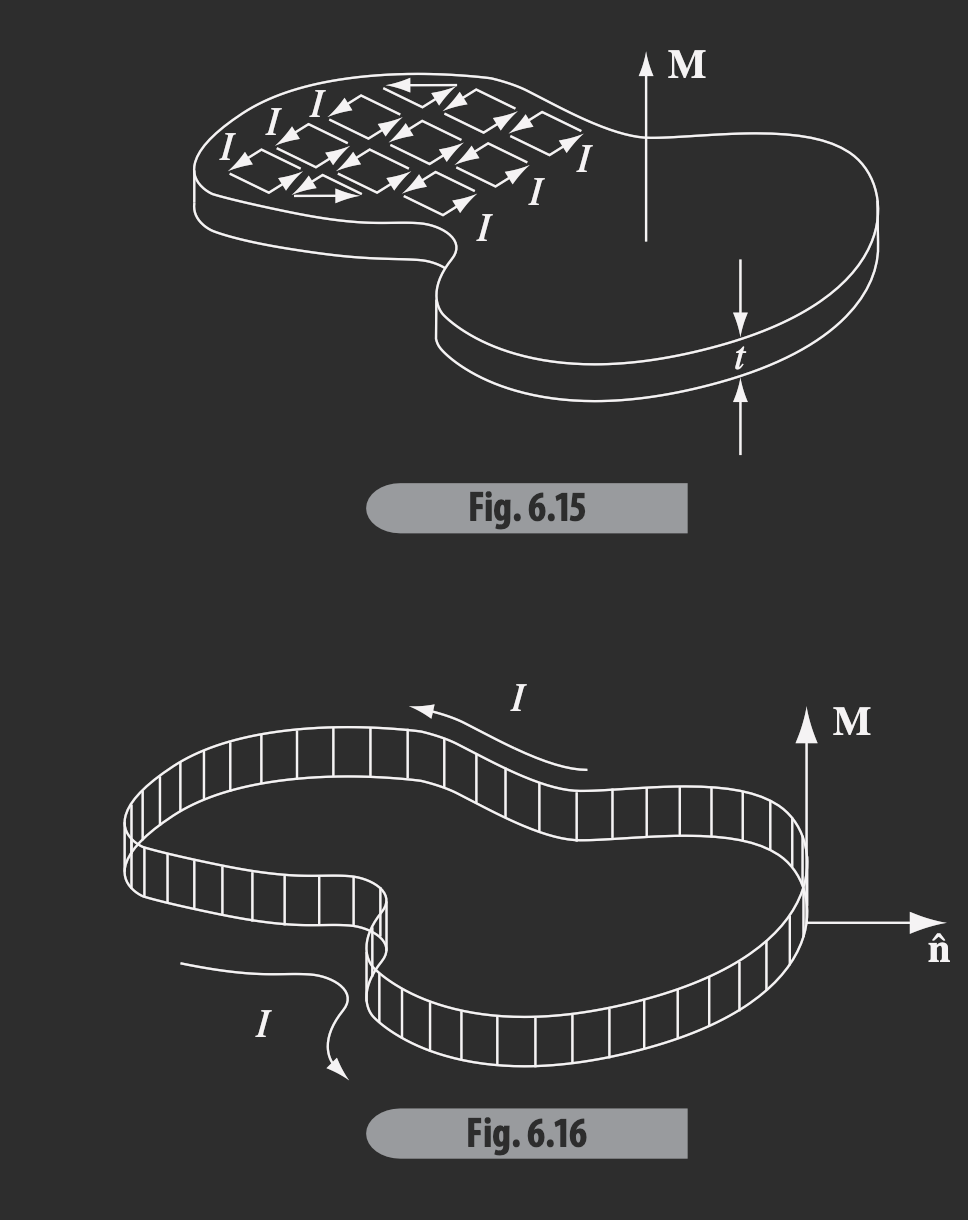
\includegraphics[width=0.4\textwidth]{fig6_15_16.png}
    \caption{Physical interpretation of bound currents}
    \label{fig:gr6_15_16}
\end{figure*}
For a magnetization $\vb M = M \vu z$ 
the little loops of current (area $a$) cancel out in the bulk of the material (of thickness $t$) but at the edges, they line up and create a train of current.
The magnitude 
\begin{align*}
    \abs{\vb m} = M at = I a \implies I_b = Mt
\end{align*}
Then the current density is
\begin{align*}
    \vb K = \vb M (\vu z \cross \vu n) = \frac{I_b}{t} (\vu z \cross \vu n)
\end{align*}
% fig6_17_18.png
\begin{figure*}[ht]
    \centering
    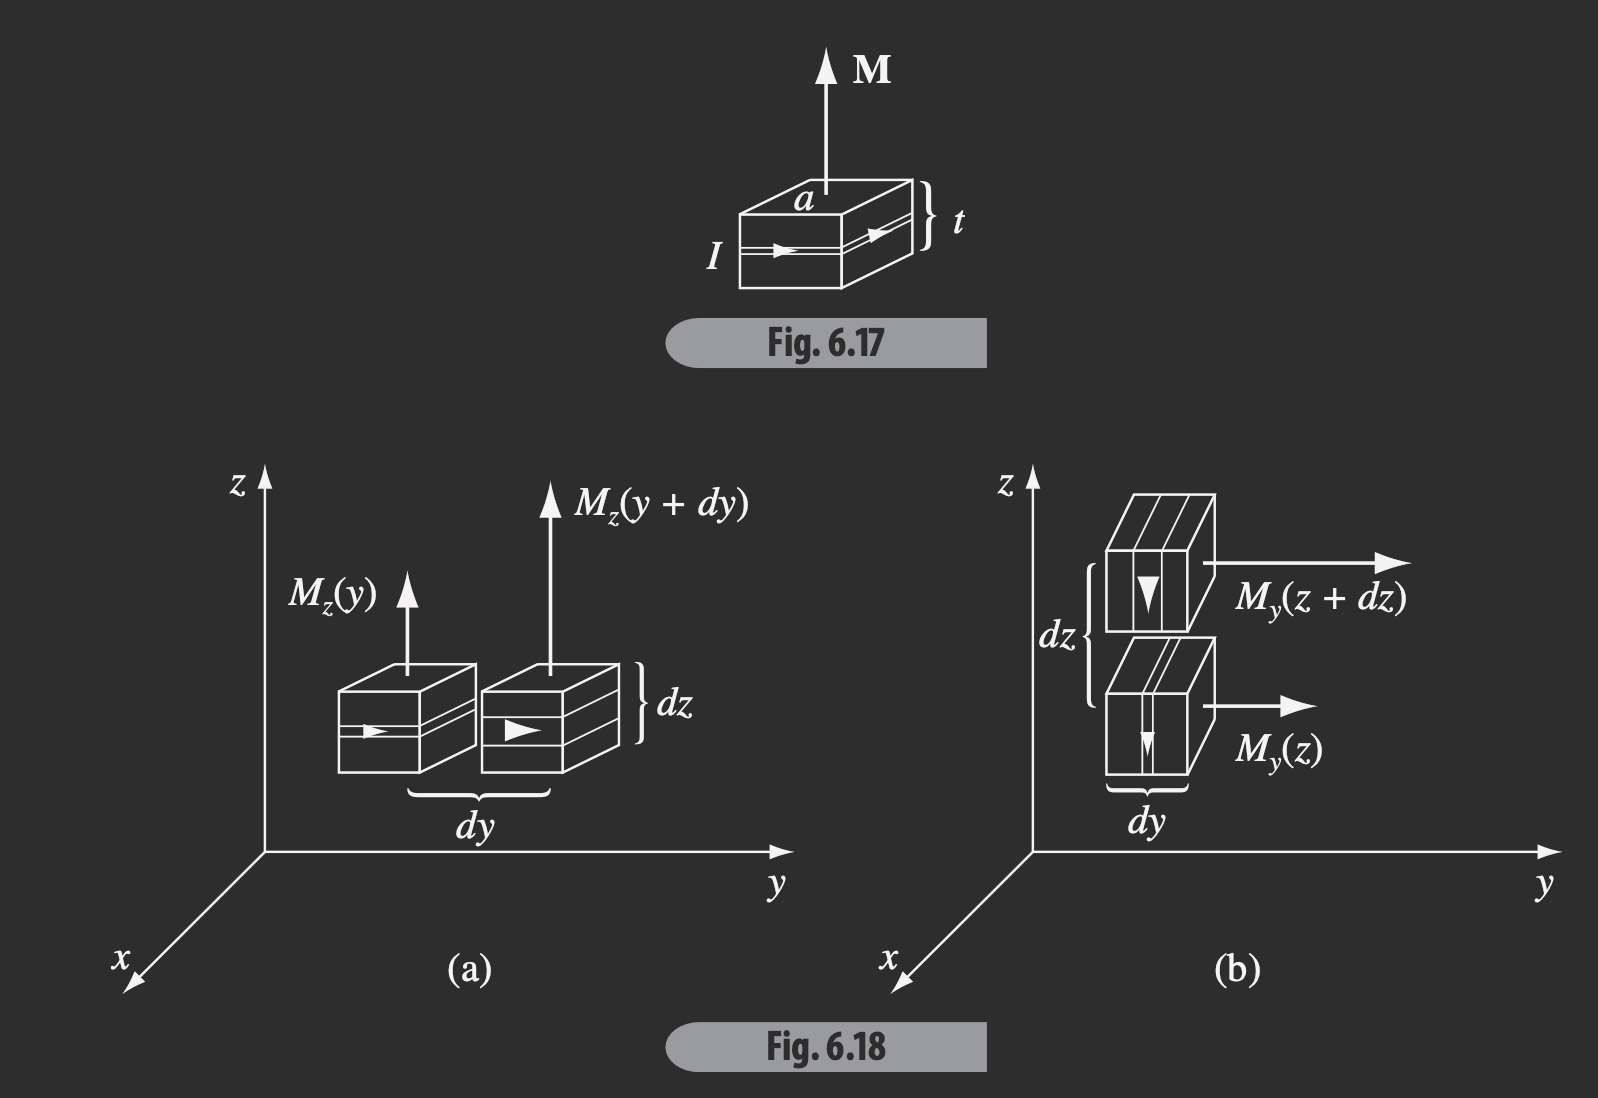
\includegraphics[width=0.4\textwidth]{fig6_17_18.png}
    \caption{Physical interpretation of bound currents}
    \label{fig:gr6_17_18}
\end{figure*}
So the current in the $x$ direction of two
adjacent loops is
\begin{align*}
    I_x = M_z (y + \dd{y}) - M_z(y) = \pdv{M_z}{y} \dd{y} 
\end{align*}
or
\begin{align*}
    J_b \eval_x = \pdv{M_z}{y}
\end{align*}
also adding the contribution from the $y$ direction
\begin{align*}
    J_b \eval_x = \pdv{M_z}{y} \vu x - \pdv{M_y}{x} \vu z \implies \vb J_b = \grad \cross \vb M
\end{align*}

\paragraph{Example} A cylinder along the $z$ axis with a uniform magnetization $\vb M = M \vu z$: Find the magnetic field $\vb B$

THe volume current is
\begin{align*}
    \vb J_b = \grad \cross \vb M = 0
\end{align*}
and the surface current is
\begin{align*}
    \vb K_b = \vb M \cross \vu n = M \vu*\phi
\end{align*}
so
\begin{align*}
    \vb B = \mu_0 n I \vu z = \mu_0 M \vu z
\end{align*}
since the surface current density is $K \sim \dv{I}{l_\perp}$

\paragraph{Example} Finding the magnetici field for a very long cylinder along $z$ with a mamgetization
\begin{align*}
    \vb M = k s^2 \vu*\phi
\end{align*}
The surface current density is
\begin{align*}
    \vb K_b = \vb M \cross \vu n = -k R^2 \vu z
\end{align*}
and the volume current density is 
\begin{align*}
    \vb J_b = \grad \cross \vb M = 3ks \vu z
\end{align*}
To find the current we can first find the total current due to the volume current density for each cross sectional area
\begin{align*}
    I_J &= \int \vb J_b \cdot \dd{\vb a} \\
    &= \int 3ks (s\dd{s}) \dd{\phi} = 2\pi k R^3
\end{align*}
then for the surface current density we integrate over the surface along the $z$ axis
\begin{align*}
    I_K &= \int -k R^2 R \dd{\phi} = -2\pi k R^3
\end{align*}
Then using Ampere's law; an amperian circular loop far away
\begin{align*}
    \oint \vb B \cdot \dd{\vb l} = \mu_0 (I_J + I_K) = 0 \implies \vb B = 0
\end{align*}
but inside the cyclinder it starts from zero and increases until we get to the surface where it drops to zero again.
\end{document}